% Exemplo de relatório técnico do IC

% Criado por P.J.de Rezende antes do Alvorecer da História.
% Modificado em 97-06-15 e 01-02-26 por J.Stolfi.
% modificado em 2003-06-07 21:12:18 por stolfi
% modificado em 2008-10-01 por cll
% modificado em 2010-03-16 17:56:58 por stolfi
% modificado em 2012-09-25 para ajustar o pacote UTF8. Contribuicao de Rogerio Cardoso
% \def\lastedit{2015-03-18 00:52:20 by bit}

\nonstopmode % PARA RODAR LATEX EM BATCH MODE
\documentclass[11pt,twoside]{article}

\usepackage{techrep-ic}

%%% SE USAR INGLÊS, TROQUE AS ATIVAÇÕES DOS DOIS COMANDOS A SEGUIR:
\usepackage[brazil]{babel}

\usepackage{makeidx}
%%% SE USAR CODIFICAÇÃO LATIN1 OU UTF-8, ATIVE UM DOS DOIS COMANDOS A
%%% SEGUIR:
%%\usepackage[latin1]{inputenc}
\usepackage[utf8]{inputenc}

%%% Para obter o tamanho de texto recomendado:
\usepackage[margin=1in]{geometry}

%%% Para colocar imagens:
\usepackage{graphicx}
\graphicspath{ {./images/} }

\usepackage{float}

\makeindex

\begin{document}

%%% PÁGINA DE CAPA %%%%%%%%%%%%%%%%%%%%%%%%%%%%%%%%%%%%%%%%%%%%%%%
%
% Número do relatório
\TRNumber{01} % Dois dígitos

% DATA DE PUBLICAÇÃO (PARA A CAPA)
%
\TRYear{18} % Dois dígitos
\TRMonth{6} % Numérico, 01-12

% LISTA DE AUTORES PARA CAPA (sem afiliações).
\TRAuthor{Ana Clara Zoppi Serpa - RA 165880
\and Bruno de Marco Apolonio - RA 195036
\and Gabriel Oliveira dos Santos - RA 197460
\and Lucas Costa de Oliveira - RA 182410
\and Vítor Mosso Dario - RA 207024}

% TÍTULO PARA A CAPA (use \\ para forçar quebras de linha).
\TRTitle{Grupo Caramelo: Sistema de gerenciamento de academia}

\TRMakeCover

%%%%%%%%%%%%%%%%%%%%%%%%%%%%%%%%%%%%%%%%%%%%%%%%%%%%%%%%%%%%%%%%%%%%%%
% O que segue é apenas uma sugestão - sinta-se à vontade para
% usar seu formato predileto, desde que as margens tenham pelo
% menos 25mm nos quatro lados, e o tamanho do fonte seja pelo menos
% 11pt. Certifique-se também de que o título e lista de autores
% estão reproduzidos na íntegra na página 1, a primeira depois da
% página de capa.
%%%%%%%%%%%%%%%%%%%%%%%%%%%%%%%%%%%%%%%%%%%%%%%%%%%%%%%%%%%%%%%%%%%%%%

%%%%%%%%%%%%%%%%%%%%%%%%%%%%%%%%%%%%%%%%%%%%%%%%%%%%%%%%%%%%%%%%%%%%%%
% Nomes de autores ABREVIADOS e titulo ABREVIADO,
% para cabeçalhos em cada página.
%

%%%%%%%%%%%%%%%%%%%%%%%%%%%%%%%%%%%%%%%%%%%%%%%%%%%%%%%%%%%%%%%%%%%%%%
% TÍTULO e NOMES DOS AUTORES, completos, para a página 1.
% Use "\\" para quebrar linhas, "\and" para separar autores.
%
\title{Caramelo: Sistema de gerenciamento de academia}

\author{
Ana Clara Zoppi Serpa
\and
Bruno de Marco Apolonio
\and
Gabriel Oliveira dos Santos
\and
Lucas Costa de Oliveira
\and
Vítor Mosso Dario
}

\date{}

\maketitle

%%%%%%%%%%%%%%%%%%%%%%%%%%%%%%%%%%%%%%%%%%%%%%%%%%%%%%%%%%%%%%%%%%%%%%

\begin{abstract}
Neste relatório abordamos o processo de desenvolvimento do projeto de MC302 ao longo deste semestre. Utilizamos a ferramenta
GitHub para controle de versões do projeto e um grupo no WhatsApp para nos comunicar e discutir o andamento do mesmo, devido às
diferenças de disponibilidade entre os membros. Dividimos o relatório em seções de acordo com as etapas de desenvolvimento
designadas pelo professor (Etapa 0, Etapa 1, Etapa 2, Etapa 3, Etapa 4 e Release Final) e descrevemos o que foi implementado/decidido
em cada uma delas e por quê.

Primeiramente, decidimos o tema e pensamos nas classes que precisaríamos, fazendo um primeiro diagrama UML. Depois, implementamos
as classes seguindo esse diagrama, mas percebemos que havia necessidades não consideradas ao elaborá-lo e coisas que poderiam ser
implementadas de uma forma diferente. Realizamos essas alterações e atualizamos o diagrama.
\end{abstract}

\clearpage
\tableofcontents

\clearpage

\section{Etapa 0: Proposta de Software}
Nessa etapa, decidimos qual seria o tema do nosso projeto e quais suas funcionalidades.
Optamos por implementar um sistema de gerenciamento de academias com cadastro de clientes, atividades
e instrutores e a associação destes, por exemplo: o cliente Gabriel faz pilates
de segunda e quarta, das 16h às 17h, e o instrutor responsável pelas aulas de pilates desse horário é o Lucas.

Escrevemos um documento descrevendo as funcionalidades que prevíamos para o sistema e entregamos para o professor.
Como elas já foram descritas no documento, aqui são mencionadas mais brevemente:

\begin{itemize}
  \item Cadastro dos clientes que frequentam a academia
  \item Alteração dos dados de um cliente já cadastrado
  \item Desativar um cliente
  \item Cadastro de atividades que a academia oferece
  \item Alteração dos dados da atividade, por exemplo, preço
  \item Remoção de uma atividade
  \item Associar/desassociar horários às atividades oferecidas
  \item Associar/desassociar clientes aos horários e atividades
  \item Cadastrar instrutores que trabalham na academia
  \item Alterar dados de um instrutor cadastrado
  \item Desativar um instrutor
  \item Consultar qual atividade possui mais clientes
  \item Consultar qual atividade possui menos clientes
  \item Consultar qual atividade tem o maior preço
  \item Consultar qual atividade tem o menor preço
\end{itemize}

Em vez de remover clientes e instrutores, optamos por desativá-los. Tivemos essa ideia pensando no seguinte cenário: um cliente
decide deixar de frequentar a academia, mas, após algum tempo, retorna. Seria prático se já tivéssemos os dados dele e bastasse
reativá-lo. O mesmo ocorre com instrutores que parem de trabalhar na academia, mas depois retornem. Ou, por exemplo, a academia
talvez tenha interesse em tentar contactar um instrutor para contratá-lo novamente, ou um cliente antigo para perguntar se ele
deseja retornar.

\section{Etapa 1: Classes do sistema}
Nessa etapa, pensamos sobre as classes e relacionamentos entre elas e construímos um diagrama UML. O professor indicou correções,
as quais realizamos em outras etapas. O diagrama a seguir está parcialmente correto e o apresentamos apenas para facilitar a
compreensão das ideias.

\begin{figure}[H]
\centering
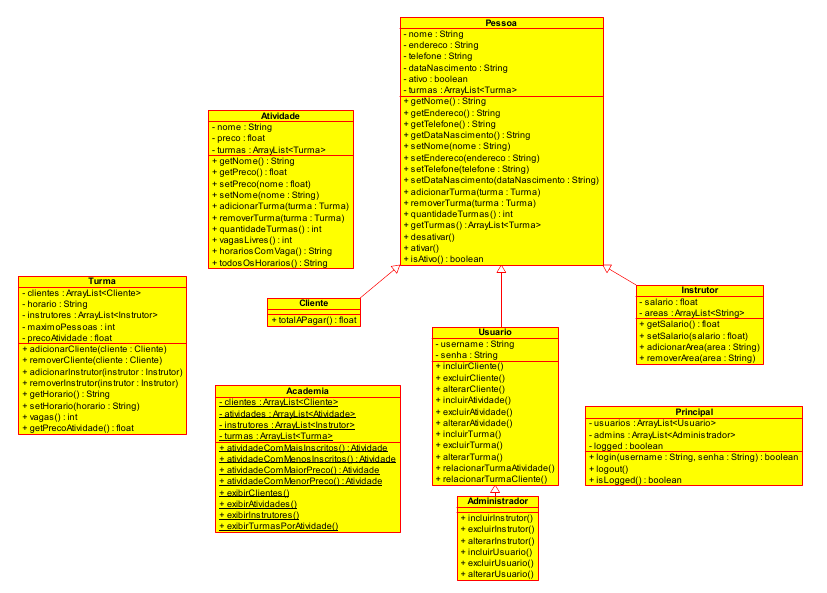
\includegraphics[width=.75\textwidth]{uml0}
\caption{Diagrama UML para a Release 0}
\end{figure}

Decidimos que o relacionamento entre cliente, horário, atividade e instrutor seria feito por meio de uma nova classe, a classe
Turma, da seguinte forma:

\begin{itemize}
  \item Uma atividade possui n turmas.
  \item Uma turma possui n clientes, n instrutores e um horário que representaremos com o tipo String.
  \item Um cliente possui n turmas, afinal, ele pode realizar várias atividades diferentes.
  \item Um instrutor possui n turmas porque ele pode dar aulas em várias turmas diferentes.
\end{itemize}

Percebemos que clientes e instrutores possuiriam nome, endereço, telefone, data de nascimento, lista de turmas e a indicação
de que estão ou não ativos no sistema como atributos em comum. Portanto, decidimos criar a classe Pessoa com esses atributos, getters e
setters
e fazer com que clientes
e instrutores fossem suas subclasses.

O cliente possui, além dos métodos e atributos da classe Pessoa, o método que calcula quanto ele precisa pagar pelas atividades
realizadas.

Como uma atividade possui n turmas, mas as turmas possuem apenas clientes, instrutores e horário, ou seja, a turma não sabe
qual é a sua atividade, decidimos, por questões de facilidade, guardar o preço da atividade na classe Turma também. Dessa forma,
para calcular quanto o cliente precisa pagar, basta iterar por sua lista de turmas e acumular os preços.

O instrutor possui, além dos métodos e atributos da classe Pessoa, um atributo salário e uma lista de áreas
(que representamos com uma lista de Strings) nas quais atua.

A classe Academia seria nossa base de dados, guardando em listas todos os clientes, instrutores, atividades e turmas do sistema
e possuindo métodos para exibí-los.

Decidimos também implementar uma etapa de login no sistema e separar os usuários entre usuários comuns e usuários administradores.
Um usuário comum poderia incluir/alterar/remover/desativar clientes, atividades e turmas, enquanto um usuário administrador
poderia fazê-lo também para instrutores e usuários. Portanto, administrador é uma subclasse de usuário.

Usuários possuem username e senha. Nessa etapa do projeto, pensamos em fazer com que Usuário fosse subclasse de Pessoa, para
guardarmos também seus dados (nome, endereço, telefone, data de nascimento).

\section{Etapa 2: Release 0}
Para essa Release, iniciamos a implementação seguindo o diagrama UML construído na Etapa 1. Criamos as classes em Java, seus métodos
e implementamos alguns deles, deixando outros vazios para serem implementados posteriormente.

\section{Etapa 3: Release 1}
Para essa Release, implementamos os métodos que, na anterior, estavam vazios. Realizamos algumas mudanças ao perceber alternativas
e necessidades não previstas.

Percebemos que não precisaríamos guardar nome, telefone, endereço e data de nascimento dos usuários do sistema, apenas username e
senha para controlar o acesso. Portanto, Usuário e Administrador deixaram de ser subclasses de Pessoa.

Decidimos, em vez de ter as classes Usuário e Administrador, ter apenas a classe Gerenciador e um enum (Permissões) para controlar
o que cada gerenciador pode fazer. O enum contém dois valores possíveis: COMUM e ADMIN. A classe Gerenciador possui métodos que
refletem as operações que o gerenciador realiza ao usar o sistema, sendo elas:
\begin{itemize}
  \item Incluir/alterar/desativar cliente.
  \item Incluir/alterar/desativar instrutor - apenas se a permissão for ADMIN.
  \item Incluir/alterar/remover um gerenciador - apenas se a permissão for ADMIN.
  \item Ver lista de gerenciadores do sistema - apenas se a permissão for ADMIN.

  As operações que podem ser realizadas apenas por ADMIN foram implementadas com um if. Se a permissão é ADMIN, os comandos
  seguintes correspondentes à operação são executados. Se a permissão não é ADMIN, é exibido um aviso.

  \item Incluir/alterar/remover atividade.
  \item Incluir/alterar/remover turma.
  \item Relacionar um cliente a uma turma, ou seja, incluí-lo naquela turma.
  \item Relacionar um instrutor a uma turma, ou seja, colocá-lo como responsável por aquela turma.
  \item Desrelacionar clientes/instrutores de uma turma.
  \item Verificar quais clientes estão em uma turma específica.
  \item Verificar quais clientes realizam uma atividade específica.
  \item Verificar quais instrutores cuidam de turmas de uma dada atividade.
  \item Consultar quantidade de clientes que realizam uma atividade.
  \item Consultar turmas de um cliente/instrutor.
\end{itemize}

A classe Principal contém uma lista (ArrayList) de gerenciadores e uma instância de  Gerenciador para guardar qual gerenciador
está logado.
Na tentativa de login, procuramos um gerenciador com o login e a senha informados pelo usuário.
Se existe, o gerenciador logado passa a ser esse que encontramos e exibimos uma mensagem (menu) com as operações possíveis.
Conforme o gerenciador digita o número correspondente à operação, chamam-se os métodos da classe Gerenciador correspondentes.
O código possui um switch case que chama os métodos correspondentes aos números das operações. Por exemplo, seja 1 a operação de
incluir um cliente: o código chama gerenciadorLogado.incluirCliente().

Os métodos da classe Gerenciador imprimem mensagens na tela solicitando os dados necessários, criando objetos a partir deles e
então chamando métodos da classe BaseDados que alteram suas listas de clientes, instrutores e atividades conforme adequado.
A classe que guardaria as listas de entidades do sistema antes se chamava Academia, mas mudamos seu nome para BaseDados.

Por exemplo, para uma inclusão de cliente, o fluxo seria o seguinte:
\begin{itemize}
  \item O método da classe Gerenciador é chamado.
  \item Um objeto Cliente é criado com base nos dados fornecidos.
  \item O método da classe BaseDados é chamado, incluindo o cliente no ArrayList de clientes que a instância de
  BaseDados possui.
\end{itemize}

Durante a implementação deles, percebemos que precisávamos de um identificador único para as turmas criadas, para que pudéssemos
associar os clientes e instrutores a elas e excluí-las. Por conta disso, acrescentamos à classe Turma um atributo ID,
a ser informado pelo
gerenciador durante a criação da turma, junto com a atividade e o horário. Também decidimos acrescentar à classe Pessoa o atributo
RG, para que fosse possível identificar unicamente cada cliente e instrutor para encontrá-los nas operações de associação a turmas,
exclusão e alteração de dados.

Para desativar um cliente, o fluxo seria o seguinte:
\begin{itemize}
  \item O método da classe Gerenciador é chamado.
  \item O RG do cliente é solicitado.
  \item O método da classe BaseDados é chamado, procurando o cliente e removendo-o caso exista.
\end{itemize}

A classe BaseDados possui, portanto, listas de clientes, atividades e instrutores, métodos para incluir/alterar/desativar/removê-los,
verificar se existem dado seu identificador único (ID de turma ou RG), relacioná-los/desrelacioná-los e verificar atividades com mais/menos
clientes e com maior/menor preço. Esses métodos são chamados pela classe Gerenciador, que realiza a interação com o usuário para conseguir
os dados necessários.

As respectivas validações também foram implementadas: por exemplo, não é possível incluir clientes de RG repetido e o sistema exibe uma mensagem
avisando sobre isso. Tentativas de desativar clientes/instrutores inexistentes também são tratadas, assim como exclusão de turmas
e atividades, entre outros casos.

Nessa etapa, as principais funcionalidades estavam prontas com suas respectivas validações, como desejado para essa release.

Atualizamos o diagrama UML para que refletisse essas mudanças, acrescentando algumas correções mencionadas
pelo professor (cardinalidades, associações, agregações etc). Não apresentamos esse diagrama neste relatório por conta de
problemas com legibilidade do texto na imagem, mas submetemos o diagrama no Google Classroom.

Também fizemos alguns protótipos de interface gráfica (telas) para o software, já que a interação com o usuário se dava apenas via console e
gostaríamos de mudar isso.

Durante a apresentação do código dessa release, o professor sugeriu que implementássemos métodos de busca, por exemplo, buscar clientes por nome/endereço/telefone e
aumentássemos a complexidade do sistema acrescentando mais conceitos de Programação Orientada a Objetos, como herança e
polimorfismo. Isso foi feito nas releases seguintes.

\section{Etapa 4: Release 2}
Seguindo as orientações do professor, implementamos métodos de busca e exploramos mais conceitos de POO no projeto. Também
fizemos mais protótipos de interface gráfica.

Além disso, removemos a interação via console com o usuário, fazendo com que os métodos da classe Gerenciador recebessem por
parâmetro os dados necessários. Fizemos isso pensando na ligação com a interface gráfica (da qual os parâmetros seriam
recuperados futuramente).
\subsection{Heranças, classes abstratas e polimorfismo}
Percebemos que não haveria instanciação de objetos da classe Pessoa no sistema, apenas de Clientes e Instrutores. Portanto, a classe
Pessoa se tornou abstrata.

Decidimos especializar mais os instrutores, tendo três tipos de instrutores: instrutores que recebem por dia trabalhado, instrutores que
recebem por hora trabalhada e instrutores que são personal trainers de clientes. Com essa mudança, clientes passaram a ter o atributo
Personal e a classe Instrutor se tornou, também, abstrata, porque todos os instrutores do sistema seriam de um desses tipos.

Decidimos que, além dos clientes comuns, teríamos clientes VIP que, além de frequentar turmas, teriam aulas a mais por semana. Mas o sistema
possui instâncias tanto de clientes como de clientes VIP, então a classe Cliente continuou concreta.

\subsection{Métodos de busca}
Implementamos, na classe Gerenciador, métodos de busca de clientes por cada um de seus atributos. O mesmo para instrutores e atividades.
Então é possível buscar clientes/instrutores por RG, nome, endereço, telefone, data de nascimento, indicação de estar ativo no sistema. No caso
dos instrutores, por área, lista de áreas e por salário também. Esses métodos retornam ArrayList<Cliente>/ArrayList<Instrutor>.

As atividades podem ser buscadas por nome, preço, lista de turmas e uma só turma. Os métodos retornam ArrayList<Atividade>.

Essas buscas podem ser realizadas tanto por gerenciadores comuns como por administradores.

{\color{red}
TODO: explicar o polimorfismo, detalhar mais o que eu escrevi acima se achar preciso.
}

\section{Release final}
{\color{red}
TODO: explicar o que foi feito.
- colocamos o login que tínhamos tirado
- mais interface gráfica
- o que mais for feito
}
\end{document}
